\documentclass[10pt]{article}
\usepackage{graphicx}
\usepackage{hyperref}
\usepackage{cite}
\usepackage{amsmath}
\usepackage{enumitem}

% wide margins
\addtolength{\oddsidemargin}{-.75in}
\addtolength{\evensidemargin}{-.75in}
\addtolength{\textwidth}{1.5in}
\addtolength{\topmargin}{-.875in}
\addtolength{\textheight}{1.75in}

\begin{document}

\title{ \textbf{0x: An open protocol for decentralized exchange on the Ethereum blockchain} }
\author{Will Warren, Amir Bandeali \\ \href{0xProject.com}{\texttt{0xProject.com}}}
\date{\today}
\maketitle 

\begin{abstract}

\noindent We describe a protocol that facilitates low friction peer-to-peer exchange of ERC20 tokens on the Ethereum blockchain. The protocol is intended to serve as an open standard and common building block, driving interoperability among decentralized applications (dApps) that incorporate exchange functionality. Trades are executed by a system of Ethereum smart contracts that are publicly accessible, free to use and that any dApp can hook into. DApps built on top of the protocol can access public liquidity pools or create their own liquidity pool and charge transaction fees on the resulting volume. The protocol is unopinionated: it does not impose costs on its users or arbitrarily extract value from one group of users to benefit another. Decentralized governance is used to continuously and securely integrate updates into the base protocol without disrupting dApps or end users. \\

\end{abstract}

\pagebreak

\tableofcontents

\pagebreak

\section{Introduction}

Blockchains have been revolutionary by allowing anyone to own and transfer assets across an open financial network without the need for a trusted third party. Now that there are hundreds\cite{coinmarketcap} of blockchain-based assets, and more being added every month, the need to exchange these assets is compounding. With the advent of smart contracts, it is possible for two or more parties to exchange blockchain assets without the need for a trusted third party. \\

\noindent Decentralized exchange is an important progression from the ecosystem of centralized exchanges for a few key reasons: decentralized exchanges can provide stronger security guarantees to end users since there is no longer a central party which can be hacked, run away with customer funds or be subjected to government regulations. Hacks of Mt. Gox, Shapeshift and Bitfinex\cite{gox,shapeshift} have demonstrated that these types of systemic risks are palpable. Decentralized exchange will eliminate these risks by allowing users to transact trustlessly - without a middleman - and by placing the burden of security onto individual users rather than onto a single custodian. \\

\noindent In the two years that have passed since the Ethereum blockchain's genesis block, numerous decentralized applications (dApps) have created Ethereum smart contracts for peer-to-peer exchange. Rapid iteration and a lack of best practices have left the blockchain scattered with proprietary and application-specific implementations. As a result, end users are exposed to numerous smart contracts of varying quality and security, with unique configuration processes and learning curves, all of which implement the same functionality. This approach imposes unecessary costs on the network by fragmenting end users according to the particular dApp each user happens to be using, destroying valuable network effects around liquidity. \\

\noindent 0x is an open protocol for decentralized exchange on the Ethereum blockchain. It is intended to serve as a basic building block that may be combined with other protocols to drive increasingly sophisticated dApps\cite{ww1}. 0x uses a publicly accessible system of smart contracts that can act as shared infrastructure for a variety of dApps, as shown in Figure \ref{fig:fig1}. In the long run, open technical standards tend to win over closed ones, and as more assets are being tokenized on the blockchain each month, we will see more dApps that require the use of these different tokens. As a result, an open standard for exchange is critical to supporting this open economy.  \\

\begin{figure}[h]
    \centering
    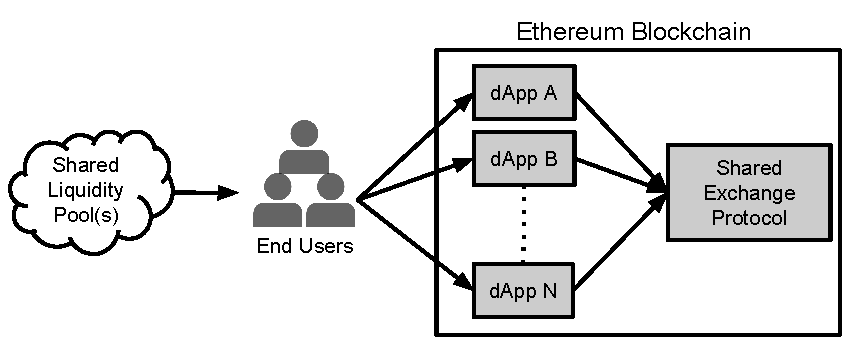
\includegraphics[width=0.7\linewidth]{../figures/fig1.pdf}
    \caption{Open protocols should be application-agnostic. Decoupling the protocol layer from the application layer provides mutual benefits for dApp developers and end users alike. }
    \label{fig:fig1}
\end{figure}

\clearpage

\pagebreak

\section{Existing Work}

Decentralized exchanges implemented with Ethereum smart contracts have failed to generate significant volume due to inefficiencies in their design that impose high friction costs on market makers. In particular, these implementations place their order books\footnote{An order book is used to publicly record the interest of buyers and sellers in a particular financial instrument. Each entry includes a reference to the interested party, the number of shares and the price that the buyer or seller are bidding/asking for the particular security. } on the blockchain\cite{maker, etheropt, augur, itt}, requiring market makers to spend gas each time they post, modify or cancel an order. While the cost of a single transaction is small, frequently modifying orders in response to evolving market conditions is prohibitively expensive. In addition to imposing high costs on market makers, maintaining an on-chain order book results in transactions that consume network bandwidth and bloat the blockchain without necessarily resulting in value transfer. \\

\noindent Automated market maker (AMM) smart contracts are proposed\cite{euler, bancor} as an alternative to the on-chain order book. The AMM smart contract replaces the order book with a price-adjustment model in which an asset's spot price deterministically responds to market forces and market participants on either side of the market trade with the AMM rather than with each other. Benefits of the AMM include availability (it is always available to act as a counterparty, though the spot price it offers may be worse than what one could get from a more traditional exchange) and ease-of-integration with external smart contracts that need to execute market orders. The deterministic nature of price-adjustment models make them “insensitive to market liquidity, meaning that trades cause prices to move the same amount in both thick and thin markets”\cite{othman2013practical}. In other words, AMMs impose artificial constraints on the supply curve. If the price-adjustment model is too sensitive, even small trades will produce large fluctuations in the spot price. If the price-adjustment model is not sensitive enough, the AMM’s bankroll will quickly be depleted by arbitrageurs. \\

% Liquidity sensitive AMMs

\noindent State channels are proposed as a means of scaling the Ethereum blockchain and reducing costs for a variety of applications - including exchange\cite{raidex} - by moving transactions off of the blockchain\cite{jcoleman, ledger}. Participants in a state channel pass cryptographically signed messages back and forth, accumulating intermediate state changes without publishing them to the canonical chain until the channel is closed. State channels are ideal for ``bar tab'' applications where numerous intermediate state changes may be accumulated off-chain before being settled by a single on-chain transaction (i.e. day trading, poker, turn-based games).  If one of the channel participants leaves the channel or attempts to cheat, there is a challenge period during which the other participant may publish the most recent message they received from the offender. It follows that channel participants must always be online to challenge a dishonest counterparty and the participants are therefore vulnerable to DDOS attacks. While state channels drastically reduce the number of on-chain transactions for specific use cases, the numerous on-chain transactions and security deposit required to open and safely close a state channel make them inefficient for one-time transactions. \\

\noindent A hybrid implementation, which we refer to as ``off-chain order relay with on-chain settlement,'' combines the efficiency of state channels with the near instant settlement of on-chain order books. In this approach, cryptographically signed orders are broadcast off of the blockchain; an interested counterparty may inject one or more of these orders into a smart contract to execute trades trustlessly, directly on the blockchain\cite{idex, etherdelta}. Friction costs are minimized for market makers because they can signal intent off-chain and transactions only occur when value is being transferred. We extend this approach by allowing anyone to act as the exchange and by making the protocol application-agnostic. \\

\clearpage

\pagebreak

\section{Specification}

Figure \ref{fig:fig2} presents the general sequence of steps used for off-chain order relay and on-chain settlement. For now we ignore a few mechanisms that will become important later.

\begin{figure}[h]
    \centering
    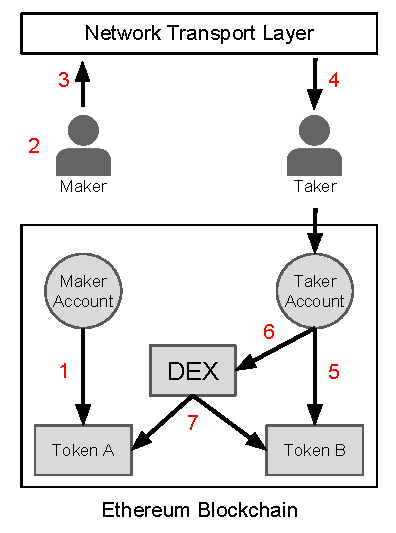
\includegraphics[width=0.4\linewidth]{../figures/fig2.pdf}
    \caption{Off-chain order relay, on-chain settlement diagram. Gray rectangles and circles represent Ethereum smart contracts and accounts, respectively. Arrows pointing to Ethereum smart contracts represent function calls; arrows are directed from the caller to the callee. Smart contracts can call functions within other smart contracts. Arrows external to the Ethereum blockchain represent information flow.  }
    \label{fig:fig2}
\end{figure}

\begin{enumerate}[noitemsep]
\item Maker approves the decentralized exchange (DEX) contract to access their balance of Token A\footnote{ See ERC20 Token in Appendix. It is possible to provide approval once and execute an unlimited number of trades thereafter. Alternatively, one can provide approval prior to - and limited to the value of - each individual trade.}.
\item Maker creates an order to exchange Token A for Token B, specifying a desired exchange rate, expiration time (beyond which the order cannot be filled), and signs the order with their private key.
\item Maker broadcasts the order over any arbitrary communication medium.
\item Taker intercepts the order and decides that they would like to fill it.
\item Taker approves the DEX contract to access their balance of Token B.
\item Taker submits the maker’s signed order to the DEX contract.
\item The DEX contract authenticates maker’s signature, verifies that the order has not expired, verifies that the order has not already been filled, then transfers tokens between the two parties at the specified exchange rate.
\end{enumerate}

\clearpage

\pagebreak

\subsection{Message Format}

Each order is a data packet containing order parameters and an associated signature. Order parameters are concatenated and hashed to 32 bytes via the Keccak SHA3 function. The order originator signs the order hash with their private key to produce an ECDSA signature.

\subsubsection{Point-to-point Orders}

Point-to-point orders allow two parties to directly exchange tokens between each other using just about any communication medium they prefer to relay messages. The packet of data that makes up the order is a few hundred bytes of hex that may be sent through email, a Facebook message, whisper or any similar service. The order can only be filled by the specified \texttt{taker} address, rendering the order useless for eavesdroppers or outside parties.

\begin{table}[h]
\centering
\caption{Message format for point-to-point orders.}
\label{table:table1}
\begin{tabular}{|l|l|l|}
\hline
\textbf{Name} & \textbf{Data Type} & \textbf{Description} \\ \hline
\texttt{version} & \texttt{address} & \begin{tabular}[c]{@{}l@{}}Address of the Exchange smart contract.\\ This address will change each time the protocol is updated.\end{tabular} \\ \hline
\texttt{maker} & \texttt{address} & Address originating the order.  \\ \hline
\texttt{taker} & \texttt{address} & Address permitted to fill the order. \\ \hline
\texttt{tokenA} & \texttt{address} & Address of an ERC20 Token contract. \\ \hline
\texttt{tokenB} & \texttt{address} & Address of an ERC20 Token contract. \\ \hline
\texttt{valueA} & \texttt{uint256} & Total units of tokenA offered by maker. \\ \hline
\texttt{valueB} & \texttt{uint256} & Total units of tokenB requested by maker. \\ \hline
\texttt{expiration} & \texttt{uint256} & Time at which the order expires (seconds since unix epoch). \\ \hline
\texttt{v} & \texttt{uint8} & ECDSA signature of the above arguments. \\ \cline{1-2}
\texttt{r} & \texttt{bytes32} & \\ \cline{1-2}
\texttt{s} & \texttt{bytes32} & \\ \hline
\end{tabular}
\end{table}

\pagebreak

\subsubsection{Broadcast Orders}

\noindent For liquid markets to emerge, there must be public locations where buyers and sellers may post orders that are subsequently aggregated into order books i.e. exchanges. Building and operating an exchange is costly and the protocol we have described so far does not provide an incentive for someone to take on such an expense. Broadcast orders solve this issue by allowing anyone to act as an exchange, maintain an order book (public or private) and charge transaction fees on all resulting liquidity. We refer to entities that host and maintain an order book as Relayers rather than exchanges. Where an exchange must build and operate proprietary infrastructure, execute trades and handle user funds, Relayers merely facilitate signalling between market participants by hosting and propagating an order book that consists of generic messages. Relayers do not execute trades on behalf of market participants as this would require market participants to trust the Relayer. Instead, Takers execute their own trades. \\

\noindent The message format for broadcast orders includes two changes to the point-to-point message format to facilitate public exchange and incentivize Relayers. First, broadcast orders do not specify a \texttt{taker} address, allowing a broadcast order to be filled by anyone that happens to intercept it. Second, broadcast orders include \texttt{feeA}, \texttt{feeB}, and \texttt{feeRecipient} parameters which specify transaction fee values and an address used by a Relayer to collect transaction fees. The exchange smart contract transfers these fees to \texttt{feeRecipient} if and when an order is filled. Figure \ref{fig:fig3} presents the sequence of steps Makers and Relayers use to negotiate transaction fees in a trustless way.

\begin{figure}[h]
    \centering
    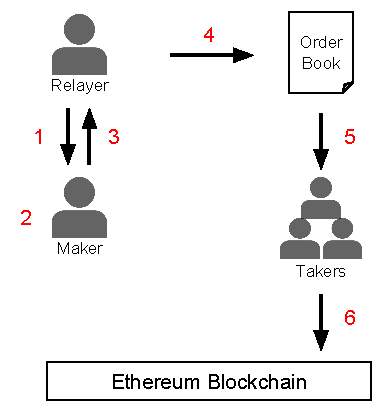
\includegraphics[width=0.4\linewidth]{../figures/fig3.pdf}
    \caption{Relayers host and maintain an off-chain order book in exchange for transaction fees. This diagram illustrates off-chain order relay and the sequence of steps used by Makers and Relayers to negotiate transaction fees in a trustless way. Transaction fees are moved from the Maker and/or Taker to the Relayer upon settlement of a trade, extending the on-chain settlement process shown in Figure \ref{fig:fig2}.  }
    \label{fig:fig3}
\end{figure}

\begin{enumerate}[noitemsep]
\item Relayer cites a fee schedule and the address they use to collect transaction fees. 
\item Maker creates an order, setting \texttt{feeA} and \texttt{feeB} to values that satisfy Relayer's fee schedule, setting \texttt{feeRecipient} to Relayer's desired recieving address and signs the order with their private key. 
\item Maker transmits the signed order to Relayer.
\item Relayer receives the order, checks that the order is valid and that it provides the required fees. If the order is invalid or does not meet Relayer's requirements, the order is rejected. If the order is satisfactory, Relayer posts the order to their order book.
\item Takers recieve an updated version of the order book that includes Maker's order.
\item Taker fills Maker's order by submitting it to the exchange contract on the Ethereum blockchain.
\end{enumerate}

\clearpage

\begin{table}[h]
\centering
\caption{Message format for broadcast orders.}
\label{table:table2}
\begin{tabular}{|l|l|l|}
\hline
\textbf{Name} & \textbf{Data Type} & \textbf{Description} \\ \hline
\texttt{version} & \texttt{address} & Address of the Exchange smart contract. \\ \hline
\texttt{maker} & \texttt{address} & Address originating the order.  \\ \hline
\texttt{tokenA} & \texttt{address} & Address of an ERC20 Token contract. \\ \hline
\texttt{tokenB} & \texttt{address} & Address of an ERC20 Token contract. \\ \hline
\texttt{valueA} & \texttt{uint256} & Total units of tokenA offered by maker. \\ \hline
\texttt{valueB} & \texttt{uint256} & Total units of tokenB requested by maker. \\ \hline
\texttt{expiration} & \texttt{uint256} & Time at which the order expires (seconds since unix epoch). \\ \hline
\texttt{feeRecipient} & \texttt{address} & Address of a Relayer. Receives transaction fees. \\ \hline
\texttt{feeA} & \texttt{uint256} & Total units of protocol token Maker pays to feeRecipient. \\ \hline
\texttt{feeB} & \texttt{uint256} & Total units of protocol token Taker pays to feeRecipient. \\ \hline
\texttt{v} & \texttt{uint8} & ECDSA signature of the above arguments. \\ \cline{1-2}
\texttt{r} & \texttt{bytes32} & \\ \cline{1-2}
\texttt{s} & \texttt{bytes32} & \\ \hline
\end{tabular}
\end{table}

\noindent While it may seem odd that the Maker is specifying the transaction fees, keep in mind that Relayers ultimately have control over which orders get posted. Therefore, if the Maker wants their order to be posted to a specific order book, they must set \texttt{feeA}, \texttt{feeB}, and \texttt{feeRecipient} to values that satisfy the Relayer associated with that order book. Since fees are negotiated off-chain, Relayers may change a fee schedule dynamically and at their own discretion (for incoming orders that haven't been signed yet, not for existing orders). Relayers may use information that is available on-chain or off-chain in setting and adjusting fees, allowing for flexible fee schedules (flat fees, percentage based, volume based, tiered, subscription models, etc). However, once the Relayer has accepted an order onto their order book, the order's fee values cannot be changed. \\

\noindent Conventional exchange services use a matching engine to fill market orders on behalf of their users and users must trust that the exchange will provide them with the best available price. Generally, users can feel assured that these regulated entities will be held accountable if they attempt to cheat or in the event that a matching engine malfunctions. For 0x protocol to remain trustless, Relayers cannot be given the ability to execute trades on behalf of Makers and Takers. Instead, Relayers can only recommend a best available price to Takers who must then independently decide to sign and send the transaction to the blockchain. This means that 0x protocol cannot support true market orders, however, a well designed web application can approximate this type of user experience. \\ 

\noindent It is important to recognize that the \texttt{feeRecipient} address can point to any arbitrary smart contract. This means that complex Relayer incentive structures can be ``plugged in'' to 0x protocol. For example, a \texttt{feeRecipient} contract could be designed to split transaction fees between multiple Relayers or distribute transaction fees across a swarm of nodes according to the level of contribution each node makes in propagating an order book within a censorship-resistant p2p network\footnote{ Development of a low-latency relay protocol that supports a fully distributed order book is being considered for the next phase of this project.}.

\clearpage

\pagebreak

\subsection{Smart Contract}

The exchange protocol is implemented within an Ethereum smart contract that is publicly accessible and free to use (no additional costs are imposed on users beyond standard gas costs). It is written in the Solidity programming language and contains two relatively simple functions: fill and cancel. The entire contract is approximately 100 lines of code and it costs approximately 90k gas to fill an order.

\subsubsection{Signature Authentication}

The exchange smart contract is able to authenticate the order originator's (Maker's) signature using the ecrecover function, which takes a hash and a signature of the hash as arguments and returns the public key that produced the signature. If the public key returned by ecrecover is equal to the \texttt{maker} address, the signature is authentic.

\begin{center}
\noindent \texttt{address publicKey = ecrecover( hash, signature( hash ) );} \\
\noindent \texttt{if ( publicKey != maker )  throw;}
\end{center}

\subsubsection{Fills \& Partial Fills}

The exchange smart contract stores a reference to each previously filled order to prevent a single order from being filled multiple times. These references are stored within a mapping; a data structure that, in this case, maps a 32 byte chunk of data to a 256 bit unsigned integer. Passing the parameters associated with an order into the Keccak SHA3 function produces a unique 32 byte hash that may be used to uniquely identify that order (the odds of a hash collision, finding two different orders with an identical hash, are practically zero). Each time an order is filled, the mapping stores the order hash and the cumulative value filled. \\

\noindent A Taker may partially fill an order by specifying an additional argument, \texttt{valueFill}, when calling the exchange smart contract's fill function. Multiple partial fills may be executed on a single order so long as the sum of the partial fills does not exceed the total value of the order.

\begin{table}[h]
\centering
\caption{Takers must provide an additional argument when attempting to fill an order.}
\label{table:table3}
\begin{tabular}{|l|l|l|}
\hline
\textbf{Name} & \textbf{Data Type} & \textbf{Description} \\ \hline
\texttt{valueFill} & \texttt{uint256} & Total units of tokenA to be filled (\texttt{valueFill} $\leq$ \texttt{valueA}). \\ \hline
\end{tabular}
\end{table}

\pagebreak

\subsubsection{Expiration Time}

An order's expiration time is specified by the Maker at the time the order is signed. The expiration time is an unsigned integer value that represents the absolute number of seconds since the unix epoch. This value cannot be changed once it has been signed. \\

\noindent Time within the Ethereum virtual machine is given by block timestamps that are set each time a new block is mined. Therefore, the expiration status of an order does not depend upon the time at which a Taker broadcasts their intention to fill an order, instead it depends upon the time at which the fill function is being executed in the EVM by a miner. A miner cannot set the block timestamp of the current block to be earlier than the timestamp of the previous block.

\subsubsection{Cancelling Orders}

An unfilled and unexpired order may be cancelled by the associated Maker via the exchange smart contract's cancel function. The cancel function maps an order's hash to the order's maximum value (\texttt{valueA}), preventing subsequent fills. Cancelling an order costs gas and, therefore, the cancel function is only intended to serve as a fallback mechanism. Typically, Makers are expected to avoid on-chain transactions by setting their order expiration times to match the frequency with which they intend to update their orders. \\

\noindent One issue with this approach is that it can create situations where a Maker attempts to cancel their order at roughly the same time a Taker is attempting to fill that same order. One of the two parties’ transactions will fail, wasting gas, depending upon the sequence in which the two transactions are mined. Uncertainty regarding the sequence in which transactions are mined could lead to undesirable outcomes at times. This uncertainty could increase if the Ethereum blockchain were to experience a significant backlog of pending transactions.

\pagebreak

\section{Protocol Token}

Cryptoeconomic protocols create financial incentives that drive a network of rational economic agents to coordinate their behavior towards the completion of a process \cite{fe1,fe2,ww1}. While 0x is fundamentally a network protocol used to facilitate signalling between buyers and sellers (rather than a cryptoeconomic protocol), it is intended to serve as an open standard for dApps that incorporate exchange functionality. Establishing and maintaining an open standard is a coordination problem that adds operational overhead for all contributing parties; coordination can be especially challenging when each party has different needs and financial incentives. Protocol tokens can align financial incentives and offset costs associated with organizing multiple parties around a single technical standard. While aligning incentives around adoption is useful, protocol tokens can be used to address a much more challenging issue: future-proofing a protocol implemented within an immutable system of smart contracts via decentralized governance.

\subsection{Decentralized Governance}

\subsubsection{Continuous Integration}

\noindent  Once an Ethereum smart contract is deployed to the blockchain its internal logic can't be changed. Therefore, to update a protocol one must deploy a completely new smart contract that either forks the network or disrupts users and processes that depend on the protocol until they ``opt-in'' to the newest version. In the context of exchange, a disruptive protocol update could invalidate all open orders and require each market participant to approve a new smart contract to access their trading balances. Alternatively, the protocol could fork into two versions that operate in parallel, neutralizing network effects created by dApp interoperability. While smart contract abstraction may be used to continuously integrate updates into a protocol without disrupting higher-level processes, such an update mechanism can also create significant security risks for end users (in the worst case, an attacker could gain access to user funds). Protocol tokens may be used to drive a decentralized update mechanism that allows for continuous integration of updates into the protocol while also protecting the protocol's users and stakeholders. \\

\noindent 0x will be deployed to the Ethereum blockchain with a fixed supply of protocol tokens that will be issued to partnering dApps and future end users. Protocol tokens will have two uses: for market participants to pay transaction fees to Relayers and for decentralized governance over updates to the protocol. Decentralized governance will be used to securely integrate updates into 0x protocol according to the process shown in Figure \ref{fig:fig4}. Initially, a simple multi-signature contract will be used for decentralized governance until a more sophisticated DAO is developed. 0x protocol and its native token will not impose unecessary costs on users, seek rent or extract value from Relayers. The protocol's smart contracts will be publicly accessible and completely free to use. No mechanisms will be put in place to benefit one group at the expense of another. \\

\begin{figure}[t]
    \centering
    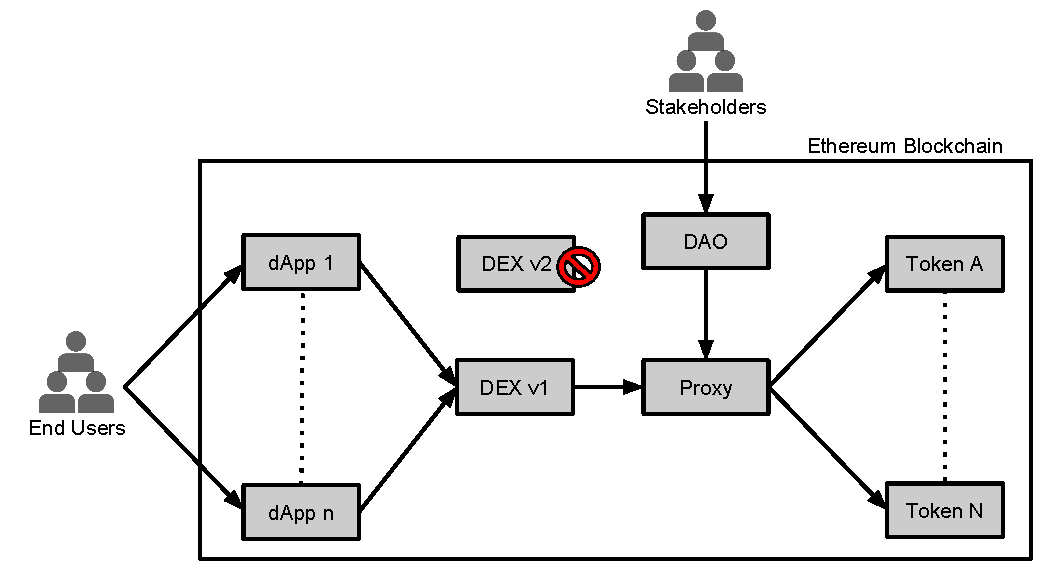
\includegraphics[width=0.8\linewidth]{../figures/fig4.pdf}
    \caption{Protocol updates may be deployed without disrupting the network through a combination of contract abstraction and decentralized governance. End users provide a Proxy contract with access to the tokens they plan on trading. Stakeholders propose and elect protocol improvements that are implemented within entirely new smart contracts (DEX v2) via a DAO. The DAO authorizes new smart contract(s) to access user tokens by adding them to the Proxy contract's whitelist and eventually unlists deprecated versions of the protocol. }
    \label{fig:fig4}
\end{figure}

\pagebreak

\subsubsection{Token Registry}

Orders consist of hexadecimal bytecode that is machine-readable but that isn't necessarily easy for a human to visually interpret. A Token Registry\footnote{https://github.com/ethereum/EIPs/issues/22} contract will be used to store a list of ERC20 tokens with associated metadata for each token: name, symbol, contract address, and the number of decimal places needed to represent a token's smallest unit (needed to determine exchange rates). The registry will serve as an “official” on-chain reference that may be used by market participants to independently verify token addresses and exchange rates before executing a trade. Since the Token Registry will serve as trusted source of information, oversight will be required to add, modify or remove tokens from the registry. 0x stakeholders will provide this oversight. While the Token Registry will make it easy for users to verify the integrity of their orders, 0x protocol can be used to trade any token that uses the ERC20 token interface. \\

\noindent In the future, the protocol's order format can be modified to facilitate human-readability. Tokens may be identified by a three character symbol registered in the Token Registry rather than by the token's contract address. The Ethereum Name Service (ENS) can  be used to identify Makers, Takers and Relayers by human-readable names, such as ``theDunkle.eth'', rather than by an account or contract address.

\clearpage

\pagebreak

\section{Summary}

\begin{itemize}[noitemsep]
\item Off-chain order relay + on-chain settlement = low friction costs for market makers + fast settlement.
\item Publicly accessible smart contracts that any dApp can hook into.
\item Relayers can create their own liquidity pools and charge transaction fees on volume.
\item Standardization + decoupling = Shared protocol layer $\rightarrow$
\begin{itemize}[noitemsep]
    \item provides interoperability between dApps
    \item creates network effects around liquidity that are mutually beneficial
    \item reduces barriers-to-entry, driving down costs for market participants
    \item eliminates redundancy, improves user experience and smart contract security
 \end{itemize}
\item Decentralized update mechanism allows improvements to be continuously and safely integrated into the protocol without disrupting dApps or end users.
\end{itemize}

\pagebreak

\section{Acknowledgements}
We would like to express our gratitude to our mentors, advisors and to the many people in the Ethereum community that have been so welcoming and generous with their knowledge. In particular, we would like to thank Joey Krug, Linda Xie and Fred Ehrsam for reviewing, editing and providing feedback on this work. We would also like to thank the organizers and community members that we've met at the Silicon Valley Ethereum Meetup including Joseph Chow, Martin Koppelmann, Rebecca Migirov, Gustav Simonsson, Grant Hummer, Tom Ding and the String Labs folks and many others.

\pagebreak

\section{Appendix}

\subsection{ERC20 Token}

\href{https://github.com/ethereum/EIPs/issues/20}{ERC20} establishes a standard contract ABI for tokens on the Ethereum blockchain and has become the de facto representation for all types of digital assets. ERC20 tokens share the same contract interface, simplifying integration with external contracts. \\ 

\noindent Core ERC20 functions include:

\begin{itemize}[noitemsep]
\item transfer(to, value)
\item balanceOf(owner)
\item approve(spender, value)
\item allowance(owner, spender)
\item transferFrom(from, to, value)
\end{itemize}

\noindent\href{https://github.com/ethereum/EIPs/issues/28}{EIP101} includes a proposal to change ether to follow the ERC20 token standard. For now, a ``wrapper'' smart contract may be used as a proxy for ERC20 ether. For reference, see the \href{https://github.com/makerdao/token-wrapper/blob/82d379769390c336abcb8ac0629d039a44d21e22/src/wrapper.sol}{Maker implementation} or the \href{https://github.com/ConsenSys/gnosis-contracts/blob/master/contracts/solidity/Tokens/EtherToken.sol}{Gnosis implementation}.

\subsection{Contract ABI}

\href{https://github.com/ethereum/EIPs/issues/50}{EIP50} proposes an extension to the contract ABI to support structs. This would allow the community to establish standard \texttt{Order} and \texttt{Signature} data structures, simplifying our contract interface and integrations with external contracts.

\subsection{Ethereum Name Service}

\href{https://github.com/ethereum/EIPs/issues/137}{EIP137} or \href{https://media.readthedocs.org/pdf/ens/latest/ens.pdf}{Ethereum Name Service} (ENS) will be used to resolve human-readable names, such as ``myname.eth,'' into machine-readable identifiers that may represent Ethereum addresses, Swarm and/or IPFS content hashes or other identifiers. It can also be used to associate metadata with names, such as contract ABIs or whois information. ENS will be used by 0x protocol to create more intuitive message formats that optionally reference Makers, Takers and Relayers by name. 

\pagebreak

\bibliography{mybib}{}
\bibliographystyle{unsrt}
   
\end{document}